\documentclass{article}
\usepackage[utf8]{inputenc}

\usepackage{fullpage}

\usepackage{tikz}
%\usetikzlibrary{calc,arrows,shapes,backgrounds,patterns,fit,decorations,decorations.pathmorphing}

\usepackage[shadow,colorinlistoftodos,textwidth=2.5cm]{todonotes}
\usepackage[final,colorlinks,hyperindex,unicode=true,pdftitle=SPAdes Manual]{hyperref}
\usepackage{url}
\usepackage{booktabs}

\def\spades{SPAdes}
\def\bh{BayesHammer}
\def\ecoli{\it E.~coli}

\usepackage{listings}
\definecolor{light-gray}{gray}{0.92}
\lstset{basicstyle=\ttfamily,framerule=0pt,frame=single,backgroundcolor=\color{light-gray}}

%\newenvironment{mycode}
%  {\begin{lstlisting}}
%  {\end{lstlisting}}

\begin{document}
\title{{\spades} 1.0.0 Manual\\{\small Revision: \today}}
\date{}
\maketitle

{\spades} stands for St.~Petersburg genome assembler.
It is intended for both single cell and standard (multicell) 
assemblies. This manual will help you to install and run
{\spades}.

We recommend to run {\spades} with pre-processing (error correction) and postprocessing (contig refinement) steps.

In our experience, the error correction tools BayesHammer and Quake work well for multicell datasets. 
However, for single cell datasets, we recommend BayesHammer rather than Quake; 
Quake was not designed for single-cell datasets, and produces inferior results. 
The performance of {\spades} on single-cell datasets deteriorates 
significantly without running BayesHammer. 

While {\spades} produces accurate assemblies, 
we recommend running NGS-Refine after {\spades} to further reduce the number of 
small errors (single nucleotide substitutions and small indels).

BayesHammer and NGS-Refine will be released after the papers describing these tools are accepted. 
Meanwhile, if you need to run these tools please contact SPAdes support (\url{spades.support@bioinf.spbau.ru}).


\renewcommand{\contentsname}{}
\tableofcontents

%\pagebreak

%\listoftodos

\pagebreak

\section{General setting}
\subsection{Notation}
{\spades} works with paired end reads.
Read size, distance, gap, and insert length are 
explained in the picture below.

\begin{center}
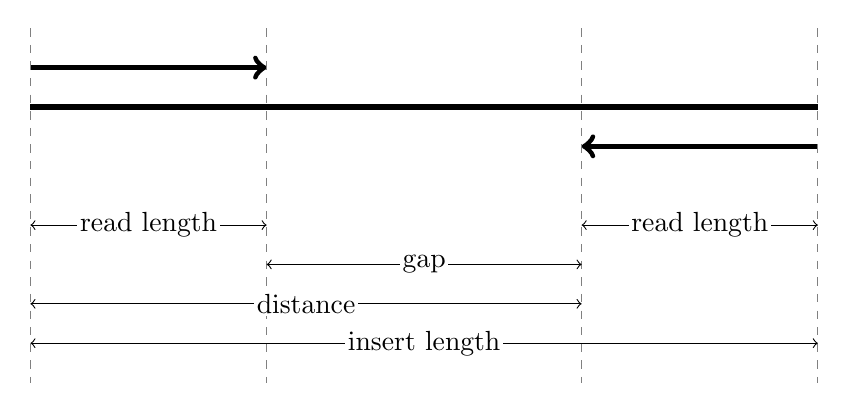
\begin{tikzpicture}
%\draw[help lines] (0,-3) grid (10,3);
\draw[line width=2pt] (0,2) -- (10,2);
\draw[line width=2pt,->] (0,2.5) -- (3,2.5);
\draw[line width=2pt,->] (10,1.5) -- (7,1.5);

\foreach \x in {0, 3, 7, 10}
  \draw[dashed,gray] (\x,3) -- (\x,-1.5);

\foreach \f/\s/\y/\t in {0/3/0.5/read length, 7/10/0.5/read length, 3/7/0/gap, 0/7/-0.5/distance, 0/10/-1/insert length}
\path[<->,draw] (\f,\y) -- node[fill=white,inner sep=1pt,rectangle] {\t} (\s,\y);
\end{tikzpicture}
\end{center}

\subsection{Config files and commands}
Config files and commands are given in gray boxes. 
%Note that the text can be copy-pasted directly from this document.
%Note also that all the links and all the colored text in the manual are clickable.
In config files, parts of lines starting with a semicolon are just comments.


\section{Getting {\spades}}
The latest version of the source code can be downloaded from\\
\url{http://bioinf.spbau.ru/spades}\\
The following code shows how to download and unpack the archived file
directly from the command line.

\begin{lstlisting}
wget http://bioinf.spbau.ru/sites/default/files/spades.zip
unzip spades.zip
\end{lstlisting}

\section{Requirements}\label{section:requirements}
\subsection{Packages}\label{subsection:packages}
%The following packages are required for using {\spades}.
The list of packages required for using {\spades} is given below.
The command
\begin{lstlisting}
sudo ./install_prerequirements
\end{lstlisting}
installs all these packages automatically if you are using {\tt apt} (advanced package tool).
%This installs all the required packages in a debian-like unix systems through {\tt apt-get install}.
If your operating system does not support {\tt apt-get} command you
need to install all the packages manually. Packages 8--14 are only needed if you are going
to use the quality tool (it measures the quality of assembly, see section~\ref{sec:running}).

\begin{center}
\begin{tabular}{rlll}
\toprule
& package & description & recommended version\\
\midrule
1 & {\tt gcc++-4.4} & GNU C Compiler & 4.4\\
2 & {\tt python2.6-dev} & Python & 2.6\\
3 & {\tt cmake} & make system & 2.6\\
4 & {\tt cmake-curses-gui} & curses based user interface for cmake & 2.6\\
5 & {\tt liblog4cxx10-dev} & logging library for {\tt C++} & \\
6 & {\tt libboost1.42-all-dev} & Boost {\tt C++} libraries & 1.42\\
7 & {\tt zlib1g-dev} & compression library & \\
%%% the following libraries are needed for quality tool
8 & {\tt java-common} & Java &\\
9 & {\tt python-matplotlib} & plotting system & \\
10 & {\tt python-numpy} & fast arrays for python & \\
11 & {\tt bioperl} & Perl tools for computational molecular biology & \\
12 & {\tt mummer} & efficient sequence alignment of full genomes & \\
13 & {\tt r-recommended} & GNU R recommended packages & \\
14 & {\tt pdftk} & tool for manipulating PDF documents & \\
\bottomrule
\end{tabular}
\end{center}

\subsection{RAM}
{\spades} requires a 64-bit Linux system.
On our test datasets,
our multi-cell {\ecoli} dataset uses 700 Mb peak memory, and our single cell
{\ecoli} dataset uses 6 Gb peak memory. 
These datasets can be found at:
\begin{itemize}
  \item multi-cell {\ecoli}:\\ \url{http://spades.bioinf.spbau.ru/spades_test_datasets/E.coli/reads/ECOLI_MC/}
  \item single-cell {\ecoli}:\\ \url{http://spades.bioinf.spbau.ru/spades_test_datasets/E.coli/reads/ECOLI_SC/}
  \item {\ecoli} reference:\\ \url{http://spades.bioinf.spbau.ru/spades_test_datasets/E.coli/reference/MG1655-K12.fasta.gz}
\end{itemize}
More datasets that {\spades} was tested on are described in section~\ref{sec:testdatasets}.

\section{Compiling}
When all the required packages are installed (see 
subsection~\ref{subsection:packages})
just run
\begin{lstlisting}
./prepare_cfg
\end{lstlisting}
in the root directory of the assembler. 
This collects all dependencies and runs {\tt cmake}.

\section{Preparing input data}
\subsection{Correcting errors in your dataset}\label{subsec:bh}
We recommend to run {\spades} with error correction step.

In our experience, the error correction tools BayesHammer and Quake work well for multicell datasets. 
However, for single cell datasets, we recommend BayesHammer rather than Quake; 
Quake was not designed for single-cell datasets, and produces inferior results. 
The performance of {\spades} on single-cell datasets deteriorates 
significantly without running BayesHammer. 

BayesHammer will be released after the papers describing the tool is accepted. 
Meanwhile, if you need to run these tools please contact SPAdes support (\url{spades.support@bioinf.spbau.ru}).

%You can do error correction with your favourite tool and then supply the resulting reads to {\spades}, but the recommended error correction tool for
%the {\spades} project is {\bh} which is also supplied in this release. To use {\bh}, you need to create a {\tt bayeshammer.info} file similar to the one
%\todo[inline]{Insert path to sample bayeshammer.info file.}
%Here are the options from the {\tt bayeshammer.info} file that you would most often want to change:
%\begin{itemize}
%\item \verb$input_working_dir$~--- directory where BayesHammer will put its temporary files and output;
%\item \verb$input_numfiles$~--- number of input files (should match the number of entries in the list below);
%\item \verb$input_paired$~--- $0$ if the input files are unpaired, 1 if paired; if $\texttt{input\_paired}=1$, \verb$input_numfiles$ should be even;
%\item \verb$input_file_0$, \verb$input_file_1$, \ldots ~--- paths to the input files;
%\item \verb$input_qvoffset$~---- PHRED quality offset in the input reads (usually $33$ or $64$);
%\item \verb$general_max_iterations$~--- number of iterations for {\bh} to run (usually, the second iteration does improve upon the first, but then it's
%diminishing returns).
%\end{itemize}
%
%After that, run {\bh} as
%\begin{verbatim}
%./assembler/build/release/hammer/main [your_bayeshammer.info_file]
%\end{verbatim}
%
%As a result, {\bh} will produce corrected files in the \verb$input_working_dir$ directory. The resulting corrected files will be named as
%\begin{verbatim}
%[iteration_num].reads.0.bad
%[iteration_num].reads.0.corrected
%[iteration_num].reads.1.bad
%[iteration_num].reads.1.corrected
%...
%\end{verbatim}
%if the input was unpaired, and
%\begin{verbatim}
%[iteration_num].reads.0.left.bad
%[iteration_num].reads.0.left.corrected
%[iteration_num].reads.0.left.unpaired
%[iteration_num].reads.0.right.bad
%[iteration_num].reads.0.right.corrected
%[iteration_num].reads.0.right.unpaired
%[iteration_num].reads.1.left.bad
%...
%\end{verbatim}
%in paired mode. The \verb$unpaired$ files contain reads that have been successfully corrected, but their paired reads have not
%(a read is not corrected successfully if it does not contain any solid $k$-mers at all). The \verb$bad$ files contain reads for which
%both the left and right read have not been successfully corrected.

%Note that {\bh} may use quite a lot of space for its temporary files (even though it gzips them by default), so choose the location
%of the working directory wisely.

\subsection{Adding your dataset to the config file}\label{subsec:datasets}
{\spades} requires paired end reads to be in separate files.
Additionally, {\spades} can use unpaired reads that normally appear after discarding one read of the paired read during error correction step.
Thus input reads should be arranged into four files: paired reads left parts, paired reads right parts, unpaired reads which originally were left parts, and
unpaired reads which originally were right parts. The first two files should contain the same number of reads, while
there are no requirements on the number of reads in the last two files (any of them can even be empty).
Files are expected to be in fasta or fastq formats and can be compressed.

In the file {\tt configs/debruijn/datasets.info} add a new entry according to the following self-explaining pattern (recall that parts of lines after from
semicolon are comments). Note that this file may contain any number of such entries.
\begin{lstlisting}
ECOLI_IS220_QUAKE
{
  first            E.coli/s_6_1.fastq.gz ; paired left
  second           E.coli/s_6_2.fastq.gz ; paired right
  single_first     E.coli/s_6_1.single.fastq.gz ; unpaired left (optional)
  single_second    E.coli/s_6_2.single.fastq.gz ; unpaired right (optional)
  RL               100 ; read length
  single_cell      false ; true if input data was obtained 
                         ; with mda (single cell) technology
  reference_genome E.coli/MG1655-K12.fasta.gz ; optional
}
\end{lstlisting}
Note that you do not need to specify the insert size or its standard deviation as {\spades}
computes them itself.

\section{Running {\spades}}\label{sec:running}
To run {\spades} type
\begin{lstlisting}
./spades.py <config.info>
\end{lstlisting}
Note that the script requires {\tt python} version~2.6.
If your default {\tt python} version is lower  type
\begin{lstlisting}
python26 ./spades.py <config.info>
\end{lstlisting}

By default (i.e., if no config file is given) {\spades} uses the file {\tt spades\_config.info}. 
Typing just {\tt ./spades.py} right after downloading and compiling runs {\spades}
on a test dataset (the first 1Kb of {\ecoli}) that is provided together with the source code.
Below we first give an example of a config file
and then explain its contents in detail.

\begin{lstlisting}																																																																																																																																																																																																																																																																																																																			
iterative_K         21 33 55
paired_mode         true 
dataset             ECOLI_IS220_QUAKE_1K
input_dir           ./data/input/
output_dir          ./data/debruijn/
measure_quality     true
output_to_console   true
\end{lstlisting}

\begin{description}
\item[{\tt iterative\_K}] specifies one or more $k$-mer (vertex) sizes.  Informally, smaller values of $k$ make the graph more connected, but at the same time more tangled, while higher values of $k$ may defragment the graph, but allow to resolving short repeats. See the paper (\cite{main}) for more details.  Note that in the configuration file, $K$ 
is the size of a vertex, while in the paper, $K$ is the size of an edge (one higher).
\item[{\tt paired\_mode}] turns on/off the repeat resolver.
\item[{\tt dataset}] is the name of the dataset as it is given in {\tt configs/debruijn/datasets.info} (see subsection~\ref{subsec:datasets}).
\item[{\tt input\_dir}] is the directory where the corresponding dataset is stored.
\item[{\tt output\_dir}] is the output directory.
\item[{\tt measure\_quality}] flag: if set to true, the quality estimation tool will be called after the assembly is performed.  The tool computes metrics such as N50, genome coverage, number of misassemblies, etc.
\item[{\tt output\_to\_console}] flag controls outputting log messages to the console.
\end{description}

\section{Understanding the output}
Results can be found in {\tt data/debruijn/DATASET\_NAME/DATE\_TIME}.
The specific directory is given at the end of the log.
Also, there is a folder containing statistics on various metrics (like N50) of the resulting contigs.
\begin{lstlisting}
All the resulting information can be found here: 
 ./data/debruijn/SAUREUS_JCVI_BH/build_02.07_19.05.56/
 * Resulting contigs are called final_contigs.fasta
 * Assessment of their quality is in quality_results/

Thank you for using SPAdes!

== Assembly finished. See the log file at: 
  ./data/debruijn/SAUREUS_JCVI_BH/build_02.07_19.05.56/spades.log
\end{lstlisting}


\section{Test datasets}\label{sec:testdatasets}
Some of the datasets that {\spades} was tested on can be found at
\url{http://bix.ucsd.edu/projects/singlecell/nbt_data.html}.
Our datasets correposnd to the followinf datasets at this page:
\begin{itemize}
\item ``ECOLI-SC'' is called ``{\ecoli}, first single cell MDA, lane 1''
\item ``ECOLI-MC'' is called ``{\ecoli} reference, lane 6''
\item ``{\it S. aureus}'' is ``{\it S. aureus}, single cell MDA, lane 7''
\item ``SAR324'' is ``{\it Deltaproteobacteria}, single cell MDA, lane 1''
\end{itemize}
The dataset ECOLI-MC may also be obtained as
``EMBL-EBI Sequence Read Archive, ascension number ERA000206''
at \url{http://www.ebi.ac.uk/ena/data/view/ERA000206&display=html}.

\section{Bug reports}
Bug reports should be sent to \url{spades.support@bioinf.spbau.ru}.


%\section{FAQ}
%\todo[inline]{Kira, Sonya, Yasha, what questions have you faced? =) }
%\subsection{How to choose the $k$-mer size?}
%\subsection{What if my question is not here?}


\bibliographystyle{plain}
\bibliography{manualbib}


\end{document}
